\documentclass{mcmthesis}

\mcmsetup{CTeX = true,   % 使用 CTeX 套装时,设置为 true
        tcn = 2215432, problem = E,
        sheet = true, titleinsheet = true, keywordsinsheet = true,
        titlepage = false, abstract = false}
\geometry{left=0.75in,right=0.75in,top=1in,bottom=1in}
\numberwithin{figure}{section}
\numberwithin{table}{section}
\numberwithin{equation}{section}
\usepackage{newtxtext}
\usepackage{lipsum}
\usepackage{palatino}
\usepackage{hyperref}
\usepackage{booktabs}
\usepackage{subfigure}
\usepackage{graphicx}
\usepackage{pythonhighlight}
\usepackage{indentfirst}%首段自动缩进
\usepackage{colortbl}
\usepackage{apacite}
\usepackage{natbib}
\usepackage{tablefootnote}
\usepackage{multicol}
%算法四部曲↓
\usepackage{algorithm}
\usepackage{algpseudocode}
\usepackage{amsmath}
\usepackage{algorithmicx}
% \usepackage{threeparttable}
\definecolor{lightBlue}{rgb}{0.867,0.922, 0.969}
\setlength{\parindent}{2em}
\title{Cultivating Strongest Guardian of Earth: Tailored Forest Management Strategies}
\setlength{\headheight}{15pt}
%伪代码
\makeatletter
\newenvironment{breakablealgorithm}
  {% \begin{breakablealgorithm}
   \begin{center}
     \refstepcounter{algorithm}% New algorithm
     \hrule height.8pt depth0pt \kern2pt% \@fs@pre for \@fs@ruled
     \renewcommand{\caption}[2][\relax]{% Make a new \caption
       {\raggedright\textbf{\ALG@name~\thealgorithm} ##2\par}%
       \ifx\relax##1\relax % #1 is \relax
         \addcontentsline{loa}{algorithm}{\protect\numberline{\thealgorithm}##2}%
       \else % #1 is not \relax
         \addcontentsline{loa}{algorithm}{\protect\numberline{\thealgorithm}##1}%
       \fi
       \kern2pt\hrule\kern2pt
     }
  }{% \end{breakablealgorithm}
     \kern2pt\hrule\relax% \@fs@post for \@fs@ruled
   \end{center}
  }
\makeatother

\begin{document}
\renewcommand{\algorithmicrequire}{\textbf{Input:}}  % Use Input in the format of Algorithm
\renewcommand{\algorithmicensure}{\textbf{Output:}} % Use Output in the format of Algorithm
\begin{abstract}

  Carbon Sequestration is one of the fundamental ways to recycle Carbon Dioxide on the Earth where 
  greenhouse effect floods. Forests, as an essential part of ecosystem, are 
  in whopping capacity of Carbon Sequestration. 
  \par
  In order to better measure the competence of Carbon Sequestration of “Earth's 
  Lung”, we develop \textbf{Binary Timber Volume Carbon Sequestration Regression Model (BTVCSR)} to 
  determine the Mass of Carbon sequestered during a period of time in the future.
  Meanwhile, a \textbf{Cellular Automata Model} is applied to 
  simulate the change of population density under natural conditions, which can 
  enter a stable stage when the \textbf{Living Environment Index} reaches \textbf{232}. 
  Sensitivity test of the Harvest Rate is carried out to find that the Subboreal 
  coniferous forest would sequester \textbf{256.83} tons of Carbon Dioxide per hectare per year 
  under an appropriate Harvest Rate of $ \bm{3\%} $ , which ranks the highest. 
  Furthermore, we compare Carbon Sequestration of different proportions of 7 kinds of wooden products 
  and predict the Mass of Carbon Sequestered in those products over 100 years 
  via \textbf{Radial Basis Function Neural Network}, which will reach around 
  \textbf{140} tons of Carbon Dioxide per hectare per year after 100 years. 
  \par
  To better understand the role Forests play both in Ecosystem and human 
  Society, we develop \textbf{Forest Carbon 
  Sequestration Multidimensional Evaluation Model (FCSME)}, which is 
  divided into \textbf{Ecological Value} and \textbf{Cultural Value}. Through establishing improved 
 \textbf{ Differential Equations of Carbon Sink Value under Multi-Tree Species Competition},
  we obtain \textbf{Intensity Thermodynamic of Sample Area Interspecific Competition}, 
  in which the highest intensity index reaches $ \bm{0.012} $ , representing the Ecological 
  Value of Competition and Carbon Sink. What's more, we develop a \textbf{Comprehensive 
  Evaluation Model of Cultural Value} based on\textbf{ Forest Hierarchy, Volume of 
  Deadwood, Proportion of Forest over Administrative Region, Forest Density} 
  and \textbf{Forest Area}, which is applicable to 4 kinds of typical classes of Forests 
  in 9 Regions of United States. By combining Ecological Value with Cultural 
  Value, we figure out that Subtropical Evergreen Broad-leaved Forest ranks the 
  top score with \textbf{0.993638 (no-harvest)} and \textbf{0.98369 (harvest)}. 
  We select and evaluate some index values to determine the transition point 
  of Strategy and help managers generate strategies.
  \par
  Application on real Forests demonstrates the correctness and robustness of our 
  Model. First of all, we apply \textbf{Autoregressive Integrated Moving Average (ARIMA)} 
  model to predict the intensity of competition, which can be used in Lotka-Volterra Model of
  different species. After that, by selecting and 
  calculating 10000 hectares of Subboreal Forests consisting of Douglars Fir and 
  Pinus Densiflora as primary types of trees in Washington State, we find that 
  the Forest will sequester \textbf{261.3} tons of Carbon Dioxide per hectare per year, 
  whose gap from reality is merely $\bm{8.1\%}$. Besides, on the occasion of increasing Rotation
  year, we find that the longer the Rotation year is, the higher Harvest Rate should be. 
  We also provide four recommendations about Rotation year and upgrade of industry for the sake of Forest Managers and Forest industries 
  to help them smoothly go through the transition period.


\begin{keywords}
Carbon Sequestration, Binary Volume Model, Lotka-Volterra Model, Forest Management, FCSME
\end{keywords}
\end{abstract}
\maketitle

\tableofcontents
  \thispagestyle{empty}
  \newpage
  \setcounter{page}{1}
%%
%%Generate the Memorandum, if it's needed.
%\memoto{\LaTeX{}studio}
%\memofrom{Liam Huang}
%\memosubject{Happy \TeX{}ing!}
%\memodate{\today}
%%\logo{\LARGE I'm pretending to be a LOGO!}
%\begin{memo}[Memorandum]
%  \lipsum[1-3]
%\end{memo}

\section{Introduction}

\subsection{Problem Restatement}
Considering that the carbon dioxide can be sequestered in both forests 
and wooden products, it's reasonable that more carbon will be stored by forests with the 
appropriate combination of the regrowth of younger forests and the wooden products.
Thus, forest managers are ought to deliberate about the balance between the value of forests 
as living tress to grow and absorb the carbon and the value of forests harvested as wooden products.
What's more, the forest managers should not only consider the factors about forests such as 
type and age of forests, geography, topography, and benefits and lifespan of forest products,
but also the conservation and diversity of wild species, recreational uses and cultural considerations.
\begin{enumerate}
    \item [1.] Design a carbon sequestration model to calculate the amount of carbon dioxide 
    sequestered by a forest and its products, which also determines what kind of manage plan is
    most efficient at sequestering carbon.
    \item [2.] Develop a decision model consisting of various ways that forests are valued (including
    carbon sequestration) for forest managers to understand the best use of a forest. Consider 
    the following questions. 
    Are there any conditions that the forests should not be harvested?
    How can the characteristics of a particular forest and its location be used 
    to determine transition points between management plans?
    \item [3.] Apply your models to various forests. Identify a forest that your decision model 
    would suggest the inclusion of harvesting in its management plan.
    How much carbon dioxide can be sequestered by this forest and its products in 100 years?
    What kind of forest management plan should be carried out for this forest? Why it's best?
    How to prolong rotation year?

    \item [4.] Some people think that we should never cut down any trees, but you've
    determined the forest which includes harvest in its management. Write a one-to-two-page
    non-technical newspaper articles to explain why your analysis including in the 
    management of the forest logging, rather than it remaining the same. Finally, your ariticle 
    should convince local community that it's the best decision for their forest.
\end{enumerate}




\section{Assumptions and Justifications}
These are necessary assumptions for simplifying the model.
\begin{enumerate}
  \item Suppose the harvested wood in warehouse doesn't corrode, meaning no change in its Carbon Sequestration;
  \item Global greenhouse effect and climate change have no influence on Forest Carbon Sequestration;
  \item Inflation is not considered when calculating Carbon sink;
  \item Only natural Forests are considered when calculating area proportion in administrative regions;
  \item Deadwood Volume, Carbon Sequestration of leaves and soil rises merely with the increase of area;
  \item Harvest is conducted evenly all around the Forest.
\end{enumerate}
\section{Overview of Our Work}

\begin{figure}[htbp]
  \centering
  \includegraphics[width = 10cm]{code&pic/框架图.pdf}
\end{figure}

\section{Notations}

\renewcommand\arraystretch{1.5}

\begin{table}[htpb!]
  \centering
  \caption{Notation Descriptions}
  \begin{tabular}{m{2.5cm}<{\centering}|m{12.5cm}<{\centering}}
  \toprule[1.5pt]
  \textbf{Symbol} & \textbf{Definition} \\ \hline
  $ \rm{DBH} $ & Diameter at Breast Height \\
  $ \beta_b $ & Conversion factor of coniferous trees\\
  $\beta_c$ & Conversion factor of broad leaf trees\\
  $ n $ & Total iteration years\\
  $ \lambda $ & Harvest rate\\
  $ M $ & Sequestered carbon mass in wooden products \\
  $ \rm{CarbonMass_f} $ & Sequestered carbon mass in forests \\
  $ \phi $ & Proportion in total product\\
  $ s $ & Scrap rate\\
  $ m $ & Decomposition rate \\
  $ K $ & Carrying Capacity \\
  $ N $ & Species population \\
  $ r $ & Population Growth Rate\\
  $ \alpha,\beta $ & Coefficient of Competition\\
  $ p $ & Rotation Years \\
  

  \bottomrule[1.5pt]
  \end{tabular}
\end{table}

\newpage

% 标题可能需要修改
\section{Binary Timber Volume Carbon Sequestration Regression Model}
\subsection{Cellular Automata based Population Size Prediction}

Cellular automata (CA) is a kind of grid dynamics model with discrete time, 
space and state, and local spatial interaction and temporal causality, which 
has the ability to simulate the space-time evolution process of complex system.
\par
Unlike general dynamical models, cellular automata are not determined by strictly 
defined physical equations or functions, but are composed of rules constructed by 
a series of models. Any model that satisfies these rules can be regarded as a cellular 
automata model. Therefore, cellular automata is a general term for a class of models, 
or a method framework. Its characteristic is that time, space and state are discrete, 
each variable only takes a finite number of states, and its state change rules are local 
in time and space.
\begin{figure}[htbp]
  \centering
  \includegraphics[width = 12cm]{code&pic/元胞自动机流程图.pdf}
  \caption{Block Diagram of typical Cellular Automata}\label{CA_Fig}
\end{figure}

The block diagram of a typical cellular automata is shown in Figure \ref{CA_Fig}, 
and the simulation result is shown in Figure \ref{CA_Result}, in which
we learn that the under the natural circumstances, the forestry population size
will reach and remain around 2100 per hectare. 

\begin{figure}[htb]
  \centering
  \includegraphics[width = 14cm]{code&pic/CA-pic.pdf}
  \caption{Result of Cellular Automation}\label{CA_Result}
\end{figure}

\subsection{Binary Timber Volume and Logistic based Carbon Sequestration Model}

In order to clearly demonstrate the amount of carbon sequestered by forests and their
products, we decide to consider the trunk volume of living trees as an estimation of 
total Volume of trees that are able to store carbon \citep{WangYan}. 
\par
\begin{figure}[htbp]
  \centering
  \includegraphics[width = 14cm]{code&pic/采伐率mindmap.pdf}
  \caption{Mind Map of Carbon Sequestration Model}
\end{figure}

\begin{algorithm}[htbp]
    \caption{Binary Timber Volume Regression of Carbon Prediction Algorithm}\label{Binary Volume Algo}
    \begin{algorithmic}[1]
      \Require
        Measurement of DBH, Height of tree ($ h $), conversion factor 
        $ \beta_c $  (coniferous) and $ \beta_b $ (broad leaf), Harvest rate $ \lambda(t) $, Carrying Capacity $ K $,
        Rotation year $ p $   
        \For{x in enumarate $ (\rm{DBH},h) $ }
        \For{k $ \gets 1$ to $ m $}
        $ P_k(x) = \frac{1}{2^kk!}\frac{d^k}{dx_k^k}(x^2-1)^k $
        \For{$ l \gets 1 $ to $m$ }

        \quad \quad Calculate $ \int_{-1}^{1}P_k(x)P_l(x)dx \gets $ Integral of Legendre Polynomials
        \If{$ k = l $}$ \int_{-1}^1P_k(x)P_l(x) = \frac{2x}{2i+1} $
        \Else $ \int_{-1}^1P_k(x)P_l(x) = 0 $   
        \EndIf 
        \EndFor
        \EndFor
        \EndFor
        
        \noindent Find $ (\rm{DBH}, h)^T $ to minimize  $ J = \int_a^b[f(\rm{DBH})+g(h)-2(x)]^2dx $
        \For{$ t \gets 1 $ to $ n $ }

        \If{$ t \mod p \equiv 0 $ }

        Regression of DBH and $ h $  

        $V_0 \gets$ Initiate

        $ V_t = a\rm{DBH}^bh^c\times Area\times \rm{Density}(\lambda, t)  $
        \EndIf
        \EndFor

        \noindent$ Area = Area_b + Area_c $

        \noindent $ \rm{CarbonMass_f} $  $= (\beta_cV_c+\beta_bV_b)+0.02\times Area_c\times 
        \frac{\rm{Density}(\lambda,t)}{K}+0.001\times Area_b \times \frac{\rm{Density}(\lambda,t)}{K}+ 70\times Area$

        \Ensure
        Carbon Dioxide Quantity of Forest = $\frac{44}{12}\times\rm{CarbonMass_f}$ 
    \end{algorithmic}
  \end{algorithm}
  For the living trees, we apply Binary Timber Volume Regression model \citep{LuoQingbang} 
  to depict their growth as shown in Algorithm \ref{Binary Volume Algo}. 
  It is significant
  to point out that $ \beta_b $ and $ \beta_c $ are two \textbf{Conversion Factors} from
  Timber Volume to Carbon Mass sequestered. Besides, the mass of carbon sequestered in
  soil and leaves can be deemed as a constant which merely depends on the area
  of coniferous and broad-leaved forests \citep{YanDeren2011}. 
  \par
  As for the wooden products, we consider $ w $ kinds of wooden products, each kind,
which decomposes at the rate of $ m_i (i = 1,\cdots, w) $, accounts for $ \phi_i$ 
of the total product mass \citep{2006Forest}. Note that the \textbf{harvest rate} $ \lambda $ and the product
proportion $ \phi $ are flexible regarding the circumstances, which are also 
the core of our forest management. And the harvest will be conducted every 
$ p $ years, which is \textbf{Rotation}. 
\par
What's more, we hold the view that 
the volume of wooden products derive from the volume of harvested trees with a certain
\textbf{Scrap Rate} $ s $. Suppose the harvested wood is stored in a well-organized
warehouse and the storage will become products in next $ p $ years, which means 
 $ \frac{1}{p} $ of all the storage will become products every year.
The complete idea is shown in Algorithm \ref{Product Algo}.


\begin{figure}[htbp]
  \begin{minipage}[htbp]{0.42\linewidth}
    The Scrap Rate is determined as following descriptions, which is also shown 
    in Figure \ref{RoundWood} on the right. There are two 
    manufacturing methods of Round Wood harvested from the forests. 
    \par
    One way is to trim the wood neatly into slabs in different shapes so that they can
    occupy most of the volume of the wood, which will be processed into softwood plywood, 
    panels and board. Meanwhile, the scrap will be manufactured into miscellaneous 
    products. It can approach the utilization rate of 81.3\%.
    \par
    The other kind of craft is to separate the bark and turn it into paper, and 
    the separated log can be processed into softwood and hardwood. The utilization 
    rate of this craft is able to reach almost 100\%.
  \end{minipage}
  \hfill
  \begin{minipage}[htbp]{0.5\linewidth}
    \begin{flushright}
      \includegraphics[width = 8.61cm]{code&pic/Roundwood cutting ways.pdf}
      \caption{Utilization Rate of Round Wood}\label{RoundWood}
    \end{flushright}
  \end{minipage}
\end{figure}


\begin{algorithm}[htbp]
  \caption{RBF Neural Network Fitting of wooden products for carbon sequestration Algorithm} \label{Product Algo}
  \begin{algorithmic}[1]
      \Require
          $ \phi $, $ s $, $ m $, $ w $ as kinds wooden products, Standardized CarbonMass and $ V $ in Algorithm1,
          Rotation year $ p $ 
      \For{$ t\gets1 $ to n}
          \For{$ i\gets1 $ to hidden\_dim}

              $ y_0 \gets Initiate $ 

              $ \hat{y_t} = \hat{y_{t-1}} + \phi_{it}V_i(t) $
          
              $ c_i\gets $ Sample CarbonMass
          
              $ \sigma_i\gets $ Z-score Normalization

              $ V_i(t) = e^{-\frac{||t-c_i||^2}{2\sigma_i^2}} $
          \EndFor

          $ M_0\gets Initiate, \quad c = t-(t\mod p)+1$ 

          \For{$ j\gets 1$ to $ w $}


          $ M_t = M_{t-1}+(1-s)\lambda \times \frac{1}{p} (\beta_cV_c(c)+\beta_bV_b(c))\times \phi_j(t)m_j(t)$ 
          \EndFor
      \EndFor
      \Ensure
      Carbon Dioxide Quantity of Wooden Products = $ \frac{44}{12} \times M_t$ 
  \end{algorithmic}
\end{algorithm}



\subsection{Results and Sensitivity Test}

We apply our model over a hypothetic forestry land with 10000 hectares, in which
the broad leaf trees takes one half and the other half is coniferous trees. Two
primary decision factors, which are harvest rate and product proportion,
are discussed by conducting sensitivity test. Detailed parameter settings can
be found in Appendix. 

% \begin{figure}[ht]
%   \begin{minipage}[htbp]{0.4\linewidth}
%     We assume that the density of the forest population follows the Logistic Model,
%     and the \textbf{Carrying Capacity of the trees} is $ K $. From the Carbon Sequestration
%     probability predicted on the right we can draw a reasonable conclusion that
%     the Logistic Model will result into chaos after 3.6 rounds of harvests. 

%   \end{minipage}
%   \hfill
%   \begin{minipage}[htbp]{0.55\linewidth}
%     \begin{flushright}
%       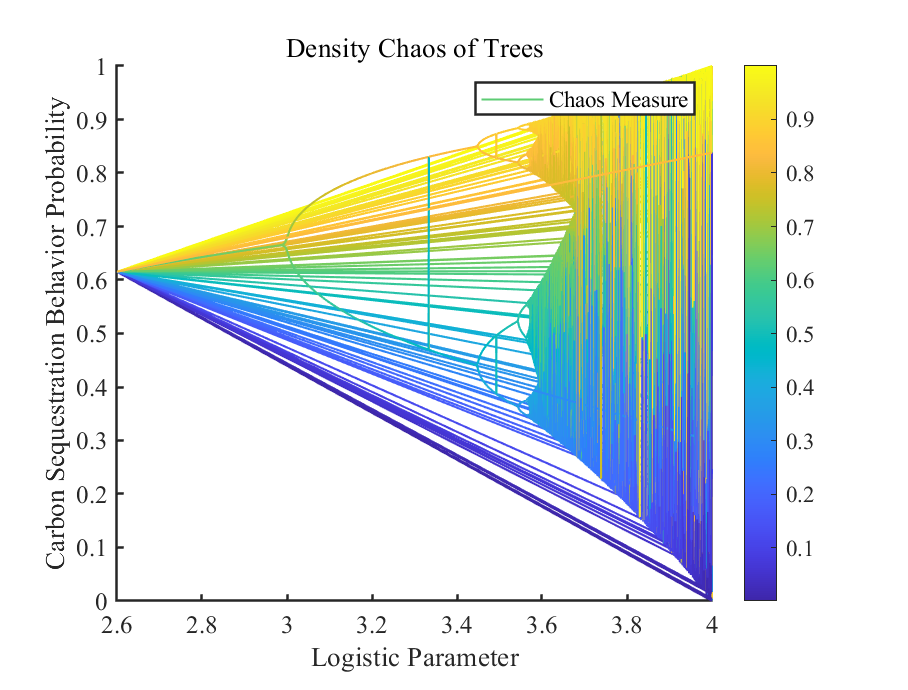
\includegraphics[width = 9cm]{code&pic/Logistic.eps}
%     \end{flushright}
%   \end{minipage}
% \end{figure}


The sensitivity test of Harvest Rate is conducted by calculating the Carbon Dioxide
sequestered by the living trees and the wooden products every 1\% of 
harvest rate from 1\% to 30\%, which can be seen in Figure \ref{Harvest Rate sensTest}.
Compared with no harvest at all, which is denoted as red line with dots on it, 
Total Carbon Sequestration under \textbf{the Harvest Rate of 0.03} ranks higher after 90 years
, reaching $ \bm{256.83} $  \textbf{tons of Carbon Dioxide per hectare per year.}
Meanwhile, it's obvious that as the Harvest Rate growing, the Total Carbon Sequestration
increases gently, bypassing those with lower Harvest Rate. Besides, if the Harvest 
Rate is too high, Total Carbon Sequestration reduces as time passes. 
\par
The sensitivity test of Product Proportion is carried out by determining the 
Carbon sequestered by wooden products under different types of product proportion
arrangement. The proportion of products with higher Decomposition Rate increases
from Type 1 to Type 5, which means in Type 5, most of the wood is consumed to manufacture
high Decomposition Rate products.The detailed proportion is shown in 
Appendix Table \ref{Types} and the result is shown in Figure \ref{Product Proportion sensTest}.
It is apparent that with Harvest Rate unchanged, the higher the proportion of
products with low Composition Rate, the higher Carbon is sequestered. \textbf{Type 5}
leads to around $ \bm{140} $\textbf{ tons of Carbon Dioxide Sequestration per hectare per year.} 

\begin{figure}[htbp]
  \centering
  \subfigure[]{
  \centering
  \includegraphics[width = 0.48\textwidth]{code&pic/采伐率.pdf}\label{Harvest Rate sensTest}
  }
  \subfigure[]{
  \centering
  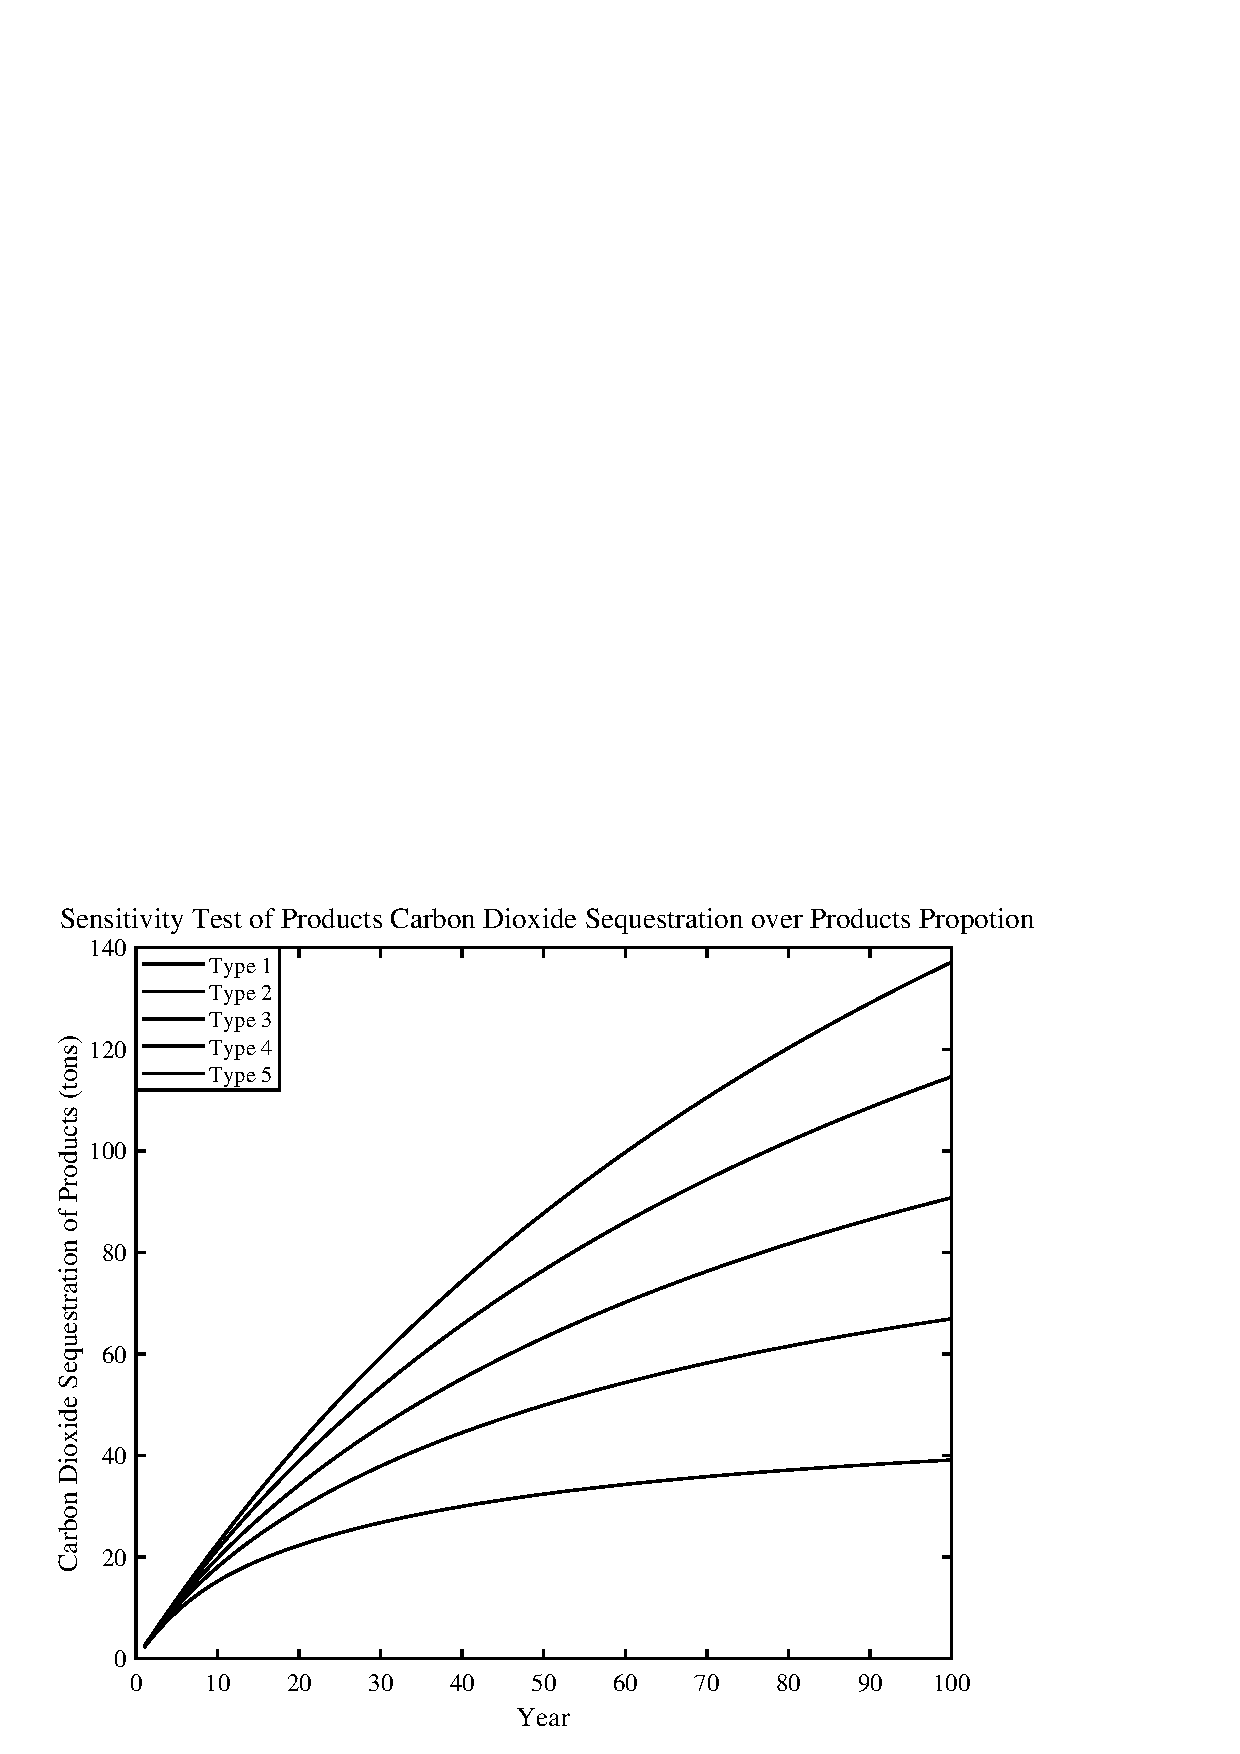
\includegraphics[width = 0.48\textwidth]{code&pic/proportion.pdf}\label{Product Proportion sensTest}
  }
\caption{Results of sensitivity test of Harvest Rate and Product Proportion}
\end{figure}

\subsection{Suggestions of Forest Management}
From what we have discussed above we can draw a very reasonable conclusion that 
there exists an appropriate Harvest Rate, which is 0.03 in our hypothetic Forest, 
that can help the Forest sequester more Carbon Dioxide after 100 years, and
the Forest managers should urge more manufactures of anticorrosive wooden products
rather than those with lower Decomposition Rate. 
\par
What's more, there are some other factors we should take into consideration when 
managing the forests. For example, the law mandates several formulae to be applied 
to calculate the minimum diameters at which species can be harvested 
sustainably \citep{lumet1993etude}. Besides, data availability, checking and 
assessment could help countries to plan and manage their forests, by giving 
concerned ministries the capacity to plan ahead, react to market shocks, help
companies when needed (possibly by also playing with costs and
tax burdens) - or even sanctioning them when parameters are not
in line with the expected values - and eventually better managing
the overall forest sector \citep{2017Cerutti}.


\section{Forest Carbon Sequestration Multidimensional Evaluation Model}


In order to comprehensively consider the multiple social interests, we add
several indexes which can fully demonstrate the impact of Forests over local 
society. 
\par
The indexes are divided into two aspects, namely \textbf{Ecological Value} and \textbf{Cultural Value}, and
Ecological Value weighs $ \bm{4.123} $  times than Cultural Value \citep{2007US}. 

\subsection{Ecological Value}
Ecological Value includes the following indexes: \textbf{Carbon Credit Benefit and 
Cost Analysis(CVal), Wooden Product Proportion, Harvest Rate} and \textbf{Interspecific 
Competition}, which will exert influence on ecological value in this Forest.
\par
CVal is a spreadsheet tool to evaluate the direct benefits and costs of Carbon 
Sequestration contracts for managed forests developed by E.M. (Ted) Bilek,
Peter Becker and Tim McAbee. By inputting a series of parameters of the Forests
such as tract size, $ \rm{CO_2} $ sequestration rate and Carbon price, CVal will
automatically come up with Average cost of trading, Net trading benefit, 
Internal Rate of Return and other important economic indexes. 
\par
Wooden Product Proportion and Harvest Rate are fully discussed above, which will not
be repeated again.
\par
Interspecific Competition is calculated by \textbf{Lotka-Volterra Model}, which is 
used to describe ecology evolution.
Suppose there are two species competing for surviving spaces, namely
Douglas Fir and Pinus Densiflora, whose population sizes are $ N_1 $ and $ N_2 $, population growth rates
are $ r_1 $ and $ r_2 $, carrying capacity $ K_1 $ and $ K_2 $ and coefficients of competition over each other 
are $ \alpha $ and $ \beta $. 
Thus, based on the Logistic growth model, the population of Douglas Fir
can be described as 
$$
  \frac{dN_1}{dt} = r_1\cdot N_1\cdot (\frac{K_1-N_1-\alpha N_2}{K_1})
$$ 
, in which $ \alpha $ is defined as a coefficients of competition of Douglas Fir over Pinus Densiflora,
representing that each Pinus Densiflora will occupy the surviving spaces of
 $ \alpha $ Douglas Firs.
 Similarly, the population of Pinus Densiflora can be described as $$
 \frac{dN_2}{dt} = r_2\cdot N_2\cdot (\frac{K_2-N_2-\beta N_1}{K_2})
 $$ 
Thus, there are four possible results for these two kinds of trees.
\begin{enumerate}
  \item [(1)] Douglas Fir wins, and Pinus Densiflora gets sidelined;
  \item [(2)] Pinus Densiflora wins, and Douglas Fir gets sidelined;
  \item [(3)] Douglas Fir and Pinus Densiflora coexist stably;
  \item [(4)] Douglas Fir and Pinus Densiflora coexist erratically.
\end{enumerate}

Whichever wins, the intensity of intraspecific competition will decline while the
intensity of interspecific competition will roar. If both species suffer high level of
intraspecific competition as well as low interspecific competition, they will stably
coexist, otherwise it leads to unstable coexistence. 
\par
Lotka-Volterra Model can be improved as follows. Suppose a second-order system can be described as the ODE below:
$$
  \frac{d^2x}{dt^2}+a_1(x,\frac{dx}{dt})\frac{dx}{dt} + a_0(x,\frac{dx}{dt})x = 0, \quad \ddot{x} = f(x,\dot{x})
$$  
Suppose $ x = x_1, \frac{dx}{dt} = x_2 $, then
$$
  \frac{dx_2}{dx_1} = \frac{f(x_1,x_2)}{x_2}
$$ 
$$
\begin{cases}
        \frac{dx_1}{dt} = x_2\\
      \frac{dx_2}{dt} =f(x_1,x_2)\\
\end{cases}
$$ 
Suppose $ x_1(t) $ denotes the position of a mass point and $ x_2(t) $ denotes the velocity of the mass point, then the 
solution of the equations depicts the movement of a point in a 2-dimension plane, and the figure of the solution is called
\textbf{Phase Diagram} in physics.
\par
Apply what we discuss above over the previous equations we can draw the improved Model:
$$
  \begin{cases}
    \frac{dr}{dt} = 2(1-\frac{r}{R})-\lambda rf, r(0) = r_0\\
    \frac{df}{dt} = -f + \lambda rf, f(0) = f_0
  \end{cases}
$$ 

\begin{figure}[htbp]
  \centering
  \subfigure[Interspecific Competition Result of Douglas Fir and Pinus Densiflora]{
  \centering
  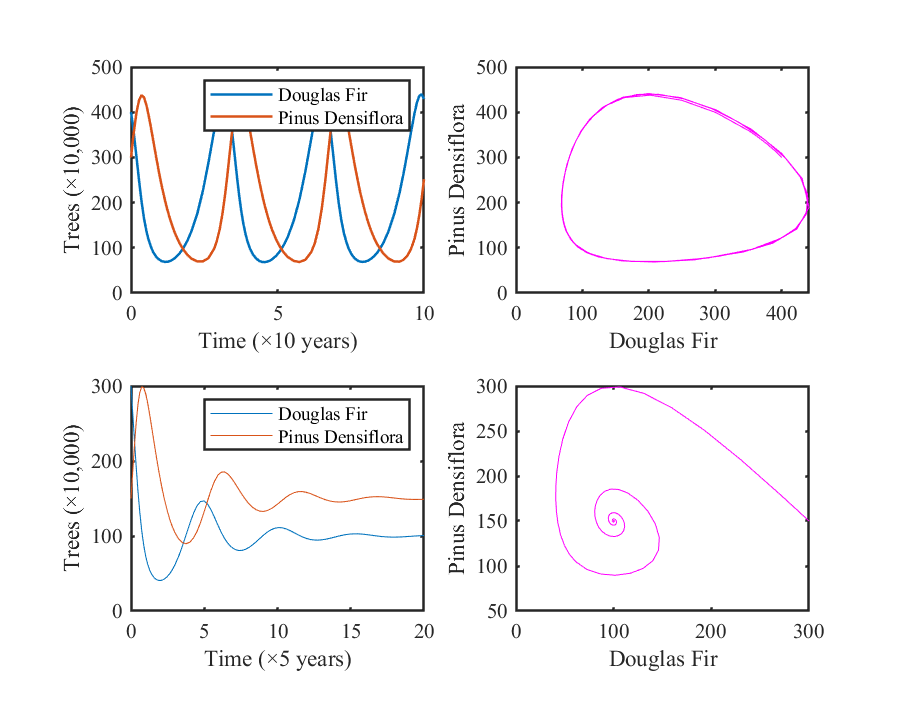
\includegraphics[width = 0.53\textwidth]{code&pic/Interspecies.eps}\label{Douglas Fir and Pinus Densiflora result}
  }
  \subfigure[Thermodynamic Diagram of Competition]{
  \centering
  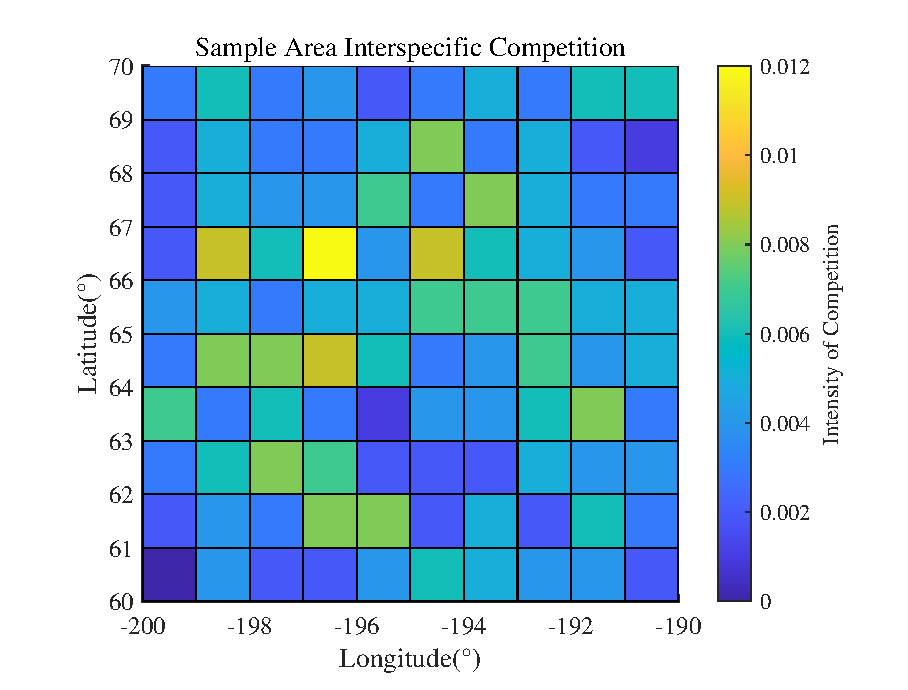
\includegraphics[width = 0.43\textwidth]{code&pic/Interspecies-matrix.eps}\label{Matrix Douglas Fir and Pinus Densiflora}
  }
\caption{Results of sensitivity test of Harvest Rate and Product Proportion}
\end{figure}

Result of the competition between Douglas Fir and Pinus Densiflora is shown in 
Figure \ref{Douglas Fir and Pinus Densiflora result}, while the thermodynamic diagram
of competition intensity between these two species can be seen in Figure \ref{Matrix Douglas Fir and Pinus Densiflora}.
In Figure \ref{Douglas Fir and Pinus Densiflora result} we can see clearly that 
there are two possible results of the interspecific competition. One is that they co-exist peacefully with their
population stabilized, while the other is that they compete fiercely, whose population fluctuate
dramatically.




\subsection{Cultural Value}

\par
In order to further demonstrate the relationship between the five indexes and 
Cultural Value, we abstract three concepts, namely Biodiversity, Development of 
Forest and Forest Influence, from the indexes. The structure of indexes related to 
Cultural Value can be clearly drawn from Figure \ref{Index_CulVal}, 
in which Proportion of Forest and Size
of Forest signify the population the Forest can influence, and Volume of Deadwood
,"an element of biodiversity and, to some extent, an indicator of forest 
management sustainability that deserves to be taken into account in inventories,
especially at the national level"\citep{rondeux2010review}, along with the 
Forest Hierarchy, which provides arboreal 
animals with more habitats, determines the Biodiversity of the Forest.
The Volume of Deadwood of the same type of forest at a similar latitude shares a similar 
constant \citep{2007US}. Size and Proportion of Forest can be searched and estimated on 
map websites, while the Forest Hierarchy is easy to search. 
\begin{figure}[htbp]
  \centering
  \includegraphics[width = 10cm]{code&pic/Model2.pdf}
  \caption{Influencing indexes of Forest Culture Value}\label{Index_CulVal}
\end{figure}

\subsection{Result and Discussion}

According to Forestry region distribution of the United States in Figure \ref{USmap}, 
we choose four typical kinds of Forests to test our evaluation model, which are
Theropencedrymion, Subboreal coniferous forest, Subtropical 
evergreen broad-leaved forest and Boreal forest. We search and calculate the index values
of these four typical Forests, and come up with their ultimate score by the method below.

\begin{figure}[htbp]
  \centering
  \includegraphics[width = 14cm]{code&pic/美国地图.pdf}
  \caption{Forest division in the United States}\label{USmap}
\end{figure}

\begin{figure}[ht]

  \hfill
  \begin{minipage}[htbp]{0.47\linewidth}
    \begin{flushleft}
      \includegraphics[width = 8cm]{code&pic/Cultural Value Composition.png}
      \caption{Radar Map of Cultural Value}\label{Radar}
    \end{flushleft}
  \end{minipage}
    \begin{minipage}[htbp]{0.45\linewidth}
      The indexes of Ecological Value are \textbf{Z-score Standardaized} and weighted summed, representing
      Ecological Value score of this kind of Forest. The indexes of Culture Value are 
      measured by \textbf{Technique for Order Preference by Similarity to an Ideal Solution (TOPSIS)}, 
      whose basic principle is to sort the indexes by detecting the distance between the 
      evaluation object and the worst solution of the optimal solution.  
      If the evaluation object is closest to the optimal solution and furthest 
      away from the worst solution, it is the best. Otherwise, it is not optimal 
      in which all index values of the optimal solution reach the optimal value 
      of all evaluation indexes and all index values of the worst solution reach 
      the worst value of all evaluation indexes. The composition of Cultural Value
      is shown in Figure \ref{Radar}.
  \end{minipage}
\end{figure}


\par
Then the scores of Ecological Value and Cultural Value are weighted added: 
$$
  \rm{TotalScore} = \frac{4.123}{5.123}\times \rm{CarbonSink} + \frac{1}{5.123}\rm{Cultural Value}
$$ 
The final scores are shown in Table \ref{ForestScore}, in which we can see that the 
Subtropical Evergreen Broad-leaved Forest ranks the highest concerning the indexes above.
There are some other interesting findings in this table. For instance, both
Theropencedrymion and Subboreal coniferous Forest approach high score in Ecological Value while 
their Cultural Values are relatively low. However, Boreal Forests are of great
significance in Cultural Value, but it doesn't help much on creating Ecological Value. 


\begin{table}[htpb!]
  \centering
  \caption{Scores of Four typical Forests} \label{ForestScore}
  \begin{tabular}{m{5.5cm}<{\centering}|m{3cm}<{\centering}|m{3cm}<{\centering}|m{3cm}<{\centering}}
  \rowcolor{lightBlue}  \textbf{Types of Forests}&\textbf{Total Score}&\textbf{Ecological Value}&\textbf{Cultural Value}\\ \hline
  \rowcolor{white} \textbf{Boreal Forest} & 0.58902 & 0.535529 & 0.809565 \\
  \rowcolor{lightBlue} \textbf{Theropencedrymion} &0.832925&0.892329&0.588001 \\
  \rowcolor{white} \textbf{Subtropical Evergreen Broad-leaved Forest} & 0.993638&0.992332 & 0.999022\\
  \rowcolor{lightBlue} \textbf{Subboreal Coniferous Forest} & 0.863477 & 0.932925 &0.577142 \\
  \end{tabular}
\end{table}

In order to figure out the conditions when Harvest Rate is 0 is recommended, 
we calculated the final scores of the four Typical Forests again without Harvest, which 
is shown in Table \ref{ForestScore-NoHarvest}. In comparison with Table \ref{ForestScore}, 
it's obvious that the all the three scores of Boreal Forest, Theropencedrymion and 
Subboreal coniferous Forest increase without harvest. 
\par
What's more, Theropencedrymion suffers severe 
Interspecific Competition without harvest; CVal of Boreal Forest increases dramatically 
without harvest; Subboreal coniferous Forest will rank higher in Culture Value if 
it's not harvested at all.
\par



\begin{table}[htpb!]
  \centering
  \caption{Scores of Four typical Forests without Harvest} \label{ForestScore-NoHarvest}
  \begin{tabular}{m{5.5cm}<{\centering}|m{3cm}<{\centering}|m{3cm}<{\centering}|m{3cm}<{\centering}}
  \rowcolor{lightBlue}  \textbf{Types of Forests}&\textbf{Total Score}&\textbf{Ecological Value}&\textbf{Cultural Value}\\ \hline
  \rowcolor{white} \textbf{Boreal Forest} & 0.704714 & 0.678393 & 0.813238 \\
  \rowcolor{lightBlue} \textbf{Theropencedrymion} &0.846885&0.908237&0.593933 \\
  \rowcolor{white} \textbf{Subtropical Evergreen Broad-leaved Forest} & 0.98369&0.986493 & 0.972135\\
  \rowcolor{lightBlue} \textbf{Subboreal Coniferous Forest} & 0.917332 & 0.947289 &0.79382 \\
  \end{tabular}
\end{table}

By further observing index values we can obtain several conditions in which banning
harvest is beneficial to in a general basis:
\begin{enumerate}
  \item [1.] Forests with \textbf{low CVal}, such as Boreal Forests;
  \item [2.] Forests with \textbf{small Deadwood Volume}, such as Subboreal Coniferous Forest;
  \item [3.] Forests with \textbf{low Forestry Density}.
\end{enumerate}


\subsection{Forestry Management Recommendations}

Location of Forests determines climate, rain, people population density, proportion 
of Forests and the probability of natural disaster, influencing Ecological Value and 
Cultural Value. Climate, rain and natural disaster are vital for the population of 
Forest, affecting Forest Density and Interspecific Competition, which are the indexes 
of Ecological value. Biodiversity and Proportion of Forest influences Cultural Value.
\par
For example, Subtropical Evergreen Broad-leaved Forest and Subboreal Coniferous Forest. 
Subtropical Evergreen Broad-leaved Forest is located in the southern United States with rich rainfall 
,relatively high temperature, solar radiation, high population density and 
biodiversity of the forest, so the ecological value is very high. Subboreal Coniferous Forest
is in the north, where the sun radiation is relatively low and latitudes is small, 
and it is relatively dry.In order to maximize the value, there must be \textbf{transition points} 
between management strategies of different Forests.
\par
According to our FCSME Model, Biodiversity, Interspecific Competition, Population 
Density and Area of Forest can be chosen to determine the transition point. After 
calculating the value of those previous indexes, Forest Managers can apply different 
strategies such as Harvest Rate, Rotation year, Crop Rotation and Rational Close 
Planting, etc. For example, when the forest population density score is 
$ [0,25],[25,50],[50,75],[75,100] $ , the logging rate will increase in turn, and the 
cutting interval time will be correspondingly compressed, and the reasonable intensity 
of dense planting will decrease in turn.
\par
Suppose population density score of Subtropical Evergreen Broad-leaved Forest is 
100 and Subboreal Coniferous Forest score is 40. So managers of Subboreal Coniferous Forest
should consider lower Harvest Rate than that of Subtropical Evergreen Broad-leaved Forest, 
increasing Rotation year and enforcing bans from cutting trees under certain diameter. 






\section{Application of Model}
So as to further reveal future Carbon Sequestration and provide managers with 
more accurate and scientific management plan, we test our Model on another forest abstracted from the forest in Washington State, which 
consists of Douglas Fir and Pinus Densiflora. Assume that their Height and DBH are
the same and they occupy $ \bm{10000} $  hectares in total. 

\subsection{Autoregressive Integrated Moving Average model}

We apply ARIMA model in order to predict the Coefficients of Competition between 
Douglas Fir and Pinus Densiflora whose \textbf{algorithm block diagram} 
is shown as Figure \ref{ARIMA_ALGO}.
\par
Under regular circumstances, the time series we obtain in the real world
  has tendency, seasonality and non-stationarity. Thus, it's vital for 
  us to transfer the non-stationary time series to stationary time series
  and make an assumption that the time series is an Auto 
  Regressive Moving Average(ARMA) series to predict the 
  future data. ARMA series is defined as follows.
  \begin{align*}
    &X_t-\phi_1X_{t-1}-\cdots -\phi_pX_{t-p} \\
    &= \epsilon_t - \theta_1\epsilon_{t-1}-\cdots-\theta_q\epsilon_{t-q}
  \end{align*}
 
$ \epsilon_1 $ is a stationary white noise whose average is zero and
deviation is $ \sigma_\epsilon^2 $;$ X_t $is an ARMA series with $ p $ and $ q $
degree, recorded briefly as $ \mathbf{ARMA}(p,q) $ series.
Akaike Information Criterion(AIC) is one of the most commonly used
criterion to determine the degree of $ \mathbf{ARMA}(p,q) $: choose 
$ p,q $ such that 
\begin{equation}\label{AIC}
    \min \mathbf{AIC} = n\ln \hat{\sigma_\epsilon^2}+ 2(p+q+1)
\end{equation}
$ n $ is the capacity of sample;$ \hat{\sigma_\epsilon^2} $ is the
estimation of $ \sigma_\epsilon^2 $ relating to $ p $ and $ q $.
\par
Suppose $ p = \hat{p}, q = \hat{q} $, such that equation(\ref{AIC}) reaches the minimum,
than we deem the series is $ \mathbf{ARMA}(\hat{p},\hat{q}) $. 
\par
Suppose $ \mathbf{ARMA}(p,q) $ series has an unknown average parameter $ \mu $,
the model becomes
$$
  \phi(B)(X_y-\mu) = \theta(B)\epsilon_t,
$$   
meanwhile, the number of unknown parameters is $ k = p+q+2 $, the AIC is:
choose $ p,q $ such that
\begin{equation}\label{AIC_unknown}
  \min \mathbf{AIC} = n\ln\hat{\sigma_\epsilon^2}+2(p+q+2).
\end{equation}  
In fact, equations (\ref{AIC}) and (\ref{AIC_unknown}) have the same minimum point $ \hat{p},\hat{q} $.
After that, we usually choose $ p = 1, q = 1 $ to make parameter estimation 
over ARMA model.


\begin{figure}[ht]
\begin{minipage}[htbp]{0.3\linewidth}
It's demonstrated that the differential operation can stabilize 
certain class of non-stationary series. And It's emphasized that 
stationary test must be conducted previously. Stationary test can 
be applied by calculating sample autocorrelation function and 
sample coefficient of partial function. 
\par
If the functions are truncated or trending to 0 (meaning being controlled
by negative index), than the series belongs to ARMA model.
\par
If at least one of the functions above is not truncated or trending to 0, than
it's not stationary.
\par

\end{minipage}
\hfill
\begin{minipage}[htbp]{0.67\linewidth}
  \begin{flushleft}
    \includegraphics[width =11cm]{code&pic/ARIMA_裁剪页面.pdf}
   \caption{Algorithm Block of ARIMA}\label{ARIMA_ALGO}
  \end{flushleft}
\end{minipage}
\end{figure}
Suppose the series is non-stationary, which can be transformed to 
a stationary series by $ d $ -degree differential operation, denoted
as $ \mathbf{ARIMA}(p,q,d) $ series,than differentiate the sample by
$ d $ -degree:
$$
  W_t = \nabla^dX_t,\quad t = d+1,\dots , n
$$ 
After that, apply stationary test on $ W_t $ and repeat steps above 
until it becomes a stationary series,then $ W_t $(which is denoted
as $ X_t $ ) complies ARMA model. 
\par

From the result of ARIMA we can see that the predicted Coefficient of Competition
between  Douglas Fir and Pinus Densiflora $ \alpha  $ and $ \beta $ is $ \bm{12.78} $  and $ \bm{11.23}$
in the future 100 years. Residual, Coefficient of Autocorrelation and Cross Coefficient
of ARIMA is shown in Figure \ref{ARIMA Res}.

\begin{figure}[htbp]
  \centering
  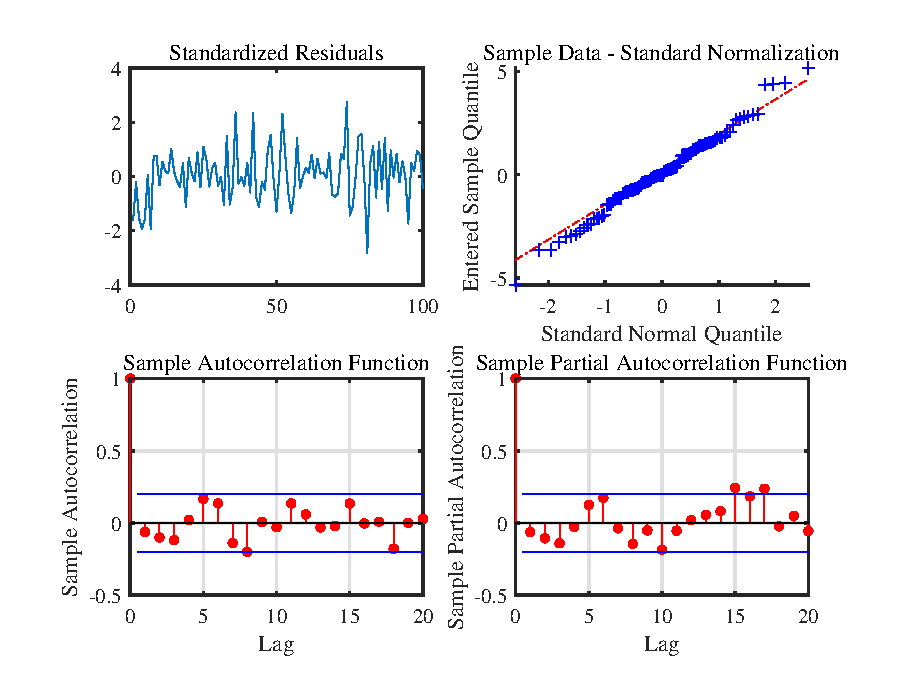
\includegraphics[width = 12cm]{code&pic/ARIMA残差&自相关互相关系数.eps}
  \caption{Residual, Coefficient of autocorrelation and cross correlation of ARIMA}\label{ARIMA Res}
\end{figure}

\newpage

\subsection{Results and Sensitivity Test}\label{applicationResult}
Under the Rotation year $ p = 3 $, we combine our first Model of Carbon Sequestration
with Lotka-Volterra Model to further simulate the change rule of Carbon Sequestration 
over 100 years. As is shown in Figure \ref{Rotation3}, the Carbon Sequestration will
approach $ \bm{2.613\times 10^6} $ tons under the Harvest Rate of 0.05.

\begin{figure}[htbp]
  \centering
  \includegraphics[width = 10cm]{code&pic/轮伐3年.pdf}
  \caption{Carbon Sequestration of $ p=3 $ }\label{Rotation3}
\end{figure}

To explore the error between our Model and the real statistics, we apply i-Tree, which
is a state-of-the-art, peer-reviewed software suite from the USDA Forest Service 
that provides urban and rural forestry analysis and benefits assessment tools. 
The i-Tree tools can help strengthen forest management and advocacy efforts by 
quantifying forest structure and the environmental benefits that trees provide.
\par
We input the area we select in Washington State into i-Tree with the Harvest Rate of 0.05
, and the result is shown in Table \ref{iTree} in Appendix. The prediction of Carbon 
Sequestration from i-Tree is $\bm{2.35197\times 10^6}$ tons. The \textbf{error rate} 
is merely $ \bm{8.9\%} $, meaning that our result of $ p = 3 $ and Harvest Rate
is 0.05 is one of the best management plans. 
\par
In order to protect interests of society during the period time of transition from 
Harvest Rate of $ 3\% $ to $ 13\% $, we test the sensitivity of Carbon Dioxide Sequestration
in Rotation Year of 1, 3, 5, 10, 13, which can be seen in Figure \ref{RotationYear}.
It's interesting that with the Rotation Years increase, the Harvest Rate under which the Forest
sequesters the most Carbon Dioxide after 100 years increases, too. If the harvest is conducted
every 13 years, then the Harvest Rate should be 0.29, which may cause severe change to the
forest on a short-term basis, but will accumulate and lead to more Carbon sequestered.

\begin{figure}[htbp]
  \centering
  \includegraphics[width = 16cm]{code&pic/轮伐图.pdf}
  \caption{Sensitivity Test of different Rotation Year}\label{RotationYear}
\end{figure}

\subsection{Discussion and Management Plans}

During the transition period, interest of two kinds of people should be taken into 
great considerations, who are Forest Managers and Forest Industries. Thus, our policy 
suggestions are as follows. 
\par
\begin{itemize}
  \item Prolong the Rotation year gradually rather than suddenly. Sudden increase of 
  Rotation year does damages to those who rely on harvesting trees. Besides, progressive, 
  predictable change creates much less resistance for managers. 
  \item Rise Harvest Rate while increasing Rotation year. Longer Rotation year means more time for Forests to recover. 
  As is discussed in section \ref{applicationResult}, managers should increase Harvest Rate to
  maintain the Carbon Sequestration and keep the economic benefits of the Forest at 
  the same level.
  \item Upgrade warehouses to improve utilization rate. With less wood corroding 
  in storage, Carbon Sequestration and economic effectiveness rise.
  \item Keep observing and tracking about circumstances of the Forest so that appropriate
  adjustments can be arranged in time.
\end{itemize}



\section{Evaluation of Model}
Our model fully considers various possible situations in Forest management, 
such as Harvest Rate and Rotation years, interspecific competition, ecological 
and cultural value, etc. and it is suitable for real conditions, indicating 
that it is a relatively perfect strategy system.

\textbf{Strength:}
\begin{enumerate}
  \item Apply the principle of Cellular Automata to design Forest cells, 
  and simulate the process of Forest natural succession, which is highly 
  practical;
  \item After comparison and verification with the actual data, it shows that the binary timber volume model can accurately calculate the carbon sequestration of a certain area of Forest, ensuring the reliability and application of the model.
  \item The interpretation and explanation of the FCSME model on the competition among multi-species Forests and Forest species in different climate zones are applicable to different Forest types across the United States, and can be further extended, and thus can serve as an effective guidance and reference for government management policies;
  \item Time series prediction model can predict the future development trend at a relatively high accuracy, consistent with the reality.
  \item Our model attributes various indicators to the evaluation of Ecological Value and Cultural Value, and considers the Forest and location characteristics to quantify the size of the Forest value in the social range, which is very beneficial to the government to determine the management strategy transition points between different Forests.


\end{enumerate}

\textbf{Weakness:}
Our models are not practiced in the formulation plan of ultra-large Forests 
and may need to be further corrected in specific practice.


\section{Conclusions}
\begin{enumerate}
  \item Through Binary Timber Volume Carbon Sequestration Regression Model and logistic model with harvesting, we can calculate the total carbon sequestration of 10000 hectares of forests and their products from 0 to 100 years. In the case of 3-year rotation, when the harvest rate is 0.03, the total carbon sequestration in the 100th year is the highest, which is 256.83 tons of carbon dioxide sequestration per hectare.
  \item While other conditions remain the same, the products with slower carbon decomposition rate account for more in the total products, and the products with faster carbon decomposition rate account for less, and the accumulated carbon sequestration in the 100th year will be more, Conversely, the less the carbon sequestration is;
  \item The established FCSME model was used to evaluate the cological cultural value of the following four forest types in the United States: Subtropical Evergreen Broad-Leaved Forest, Subboreal Coniferous Forest, Boreal Forest and Theropencedrymion, and weighted and ranked according to the weight of 4.123:1, In both cases of cutting and no cutting, Its rankings are as follows: subtropical evergreen broad-leaved forest> Subboreal Coniferous Forest> Theropencedrymion> Boreal Forest. In the case of harvesting, scores were 0.993638, 0.863477, 0.832925, 0.58902, the ranking remained unchanged without harvesting, and the scores of other forests increased except that of subtropical evergreen broad-leaved forest.
  \item We tested the sensitivity of carbon sequestration in 100 years to rotations, and found that when the rotation year were extended to 1,3,5 and 10 years respectively, the harvest rate corresponding to the highest carbon sequestration in the 100th year would increase correspondingly, which were 0.02,0.1,0.22 and 0.29, respectively.
\end{enumerate}


\newpage

\phantomsection\addcontentsline{toc}{section}{Harvesting Trees is Good For All!}\tolerance=500

\memodate{\today}

\begin{memo}[Harvesting Trees is Good For All!]

  \begin{figure}[ht]
    \hfill
    \begin{minipage}[htbp]{0.475\linewidth}
      \indent\setlength{\parindent}{1em}
      \par
      Harvesting trees has become a symbol against environmental protection in recent decades
      thanks to the over whelming propaganda of tropical rain forests falling down, causing
      great damage to our ecosystem and so on. However, there is one thing that needs to be 
      claimed: Appropriate harvest of trees is good for all! It's not only beneficial to
      the environment and the ecosystem, but also good for us human-beings, in no matter
      short or long term.
      \par
      As is kwon to all, climate change has become one of the top agendas concerning the 
      future of humanity, which is primarily caused by greenhouse gases, in which carbon
      dioxide ranks very high. Plants can absorb carbon dioxide vented by animals or released
      by burning fossil fuels, and forests are playing a significant role in sequestering
      carbon from atmosphere, preventing it from making greenhouse effect even worse. 
      \par
      \includegraphics[width = 8cm]{code&pic/大循环.pdf}
      \par
      Some people may wonder why should we harvest trees if they are so important in sequestering
      carbon dioxide? There are two reasons for this.  
    \end{minipage}
    \hfill
    \begin{minipage}[htbp]{0.475\linewidth}
      \indent\setlength{\parindent}{1em}
      \par
      First of all, if we cut those mature trees whose capacity of sequestering carbon is declining, 
      we make surviving room for those younger trees who sequester more carbon 
      than those harvested during the same period of time. 
      Besides, wooden products made of harvested trees can reserve the carbon they 
      sequestered much more longer than the deadwood do, because people are quite careful
      about preventing corrosion from their furniture and house. 
      Thus, harvesting trees helps Sequester more carbon.
      \par
      The second reason why cutting down trees is better than not cutting down trees is that 
      cutting down trees is better for people.
      \par
      In social and economic perspective, forest harvest brings larger profit to many 
      industries. The storage, processing, transportation and transaction of wooden 
      products profoundly stimulate economic growth of our society, without which 
      there will be lots of unemployment.
      \par
      What's more, wooden products facilitate our daily life, lifting people's quality 
      of life. Generally speaking, the quality of mature trees in forests is better 
      than that of planted trees, and they will have an advantage in terms of wood
      density, hardness, flatness and longevity. With most people now more interested 
      in product quality, wood sources from forests will become more popular in the 
      market and the public
      \par
      In a nut shell, harvesting trees benefits both natural and social environment 
      enormously. Thus, appropriate forest harvest is the best decision under the 
      consideration of the balance of environmental protection, economic benefits 
      and quality of life. Hopefully we can be more tolerant of harvesting trees and 
      establish a better home for all of us!

    \end{minipage}

  \end{figure}
\end{memo}




\newpage

%这一行是用来将Reference添加到目录的
\phantomsection\addcontentsline{toc}{section}{Refence}\tolerance=500

\bibliographystyle{apacite}
\bibliography{reference.bib}


\lhead{\small\sffamily \team}
% \rhead{\small\sffamily Page \thepage\ }

\newpage

\begin{appendices}

\textbf{Parameter Settings of hypothetic Forest:}

$ a=0.00006303;
D1=0.25;
D2=0.35;
b=1.8218;
H1=25;
H2=10;
c=1.0282;$

$
N1=5000;
N2=5000;
s=0.001;%折损率
$

$
d=[0.125984252 0.031496063 0.251968504 0.503937008 0.062992126 0.015748031 
0.007874016];
 $ 
 \par

 \textbf{Decomposition conditions of wooden products:}
\begin{figure}[htbp]
  \centering
  \includegraphics[width = 14cm]{code&pic/产品腐败数据.pdf}
\end{figure}

\begin{table}[htbp]
  \caption{Proportion of Products in different Types}\label{Types}
  \begin{tabular}{c|ccccc}
  \textbf{Types of wooden production}                        & \textbf{Type1} & \textbf{Type2} & \textbf{Type3} & \textbf{Type4} & \textbf{Type5} \\ \hline
  \cellcolor[HTML]{FFFFFF}\textbf{Softwood lumber}      & 0.125984252    & 0.178571429    & 0.142857143    & 0.107142857    & 0.031496063    \\
  \cellcolor[HTML]{FFFFFF}\textbf{Hardwood lumber}      & 0.031496063    & 0.107142857    & 0.142857143    & 0.178571429    & 0.125984252    \\
  \cellcolor[HTML]{FFFFFF}\textbf{Softwood plywood}      & 0.251968504 & 0.214285714 & 0.142857143 & 0.071428571 & 0.015748031 \\
  \cellcolor[HTML]{FFFFFF}\textbf{Oriented strandboard} & 0.503937008    & 0.25           & 0.142857143    & 0.035714286    & 0.007874016    \\
  \cellcolor[HTML]{FFFFFF}\textbf{Non-structural panels} & 0.062992126 & 0.142857143 & 0.142857143 & 0.142857143 & 0.062992126 \\
  \textbf{Miscellaneous products}                       & 0.015748031    & 0.071428571    & 0.142857143    & 0.214285714    & 0.251968504    \\
  \textbf{Paper}                                        & 0.007874016    & 0.035714286    & 0.142857143    & 0.25           & 0.503937008   
  \end{tabular}
\end{table}

\newpage

\begin{table}[ht]
  \caption{Result of i-Tree}\label{iTree}
  \begin{tabular}{
  >{\columncolor[HTML]{FFFFFF}}c |
  >{\columncolor[HTML]{FFFFFF}}c 
  >{\columncolor[HTML]{FFFFFF}}c 
  >{\columncolor[HTML]{FFFFFF}}c 
  >{\columncolor[HTML]{FFFFFF}}c 
  >{\columncolor[HTML]{FFFFFF}}c 
  >{\columncolor[HTML]{FFFFFF}}c }
  \textbf{Year} & \textbf{Products(C)} & \textbf{Landfill(C)} & \textbf{Stored(C)} & \textbf{Energy(C)} & \textbf{Emissions(C)} & \textbf{Total(C)} \\ \hline
  0       & 105.543 & 0      & 105.543 & 48.085 & 29.434 & 288.605 \\
  10      & 47.065  & 22.474 & 69.539  & 68.35  & 45.174 & 252.602 \\
  20      & 30.58   & 27.544 & 58.125  & 73.748 & 51.142 & 241.139 \\
  30      & 24.084  & 28.868 & 52.952  & 75.524 & 54.54  & 235.968 \\
  40      & 19.916  & 29.601 & 49.517  & 76.66  & 56.975 & 232.669 \\
  50      & 16.846  & 30.15  & 46.996  & 77.299 & 58.72  & 230.011 \\
  60      & 14.462  & 30.746 & 45.208  & 77.665 & 60.142 & 228.223 \\
  70      & 12.627  & 31.206 & 43.833  & 77.848 & 61.334 & 226.848 \\
  80      & 11.022  & 31.666 & 42.688  & 78.031 & 62.297 & 225.704 \\
  90      & 9.826   & 32.078 & 41.905  & 78.031 & 63.123 & 224.963 \\
  100     & 8.77    & 32.449 & 41.219  & 78.031 & 63.812 & 224.281 \\
  Average & 23.874  & 28.269 & 52.143  & 74.774 & 56.137 & 235.197
  \end{tabular}
  \end{table}

\textbf{\textcolor[rgb]{0.98,0.00,0.00}{Input matlab source:}}
\lstinputlisting[language=Matlab]{code&pic/Untitled5.m}

\end{appendices}


\end{document}

